% Written by Ava Hoffman
% Please use as you like, but it would be nice if you credited me :)
% 
% I find it easiest to edit and compile this in RStudio - won't work with TexShop due to
% embedded ggplot plots.

%%%%%%%%%%%%%%%%%%%%%%%%%%%%%%%%%%%%%%%%%
\documentclass{resume}\usepackage[]{graphicx}\usepackage[]{color}
% maxwidth is the original width if it is less than linewidth
% otherwise use linewidth (to make sure the graphics do not exceed the margin)
\makeatletter
\def\maxwidth{ %
  \ifdim\Gin@nat@width>\linewidth
    \linewidth
  \else
    \Gin@nat@width
  \fi
}
\makeatother

\definecolor{fgcolor}{rgb}{0.345, 0.345, 0.345}
\newcommand{\hlnum}[1]{\textcolor[rgb]{0.686,0.059,0.569}{#1}}%
\newcommand{\hlstr}[1]{\textcolor[rgb]{0.192,0.494,0.8}{#1}}%
\newcommand{\hlcom}[1]{\textcolor[rgb]{0.678,0.584,0.686}{\textit{#1}}}%
\newcommand{\hlopt}[1]{\textcolor[rgb]{0,0,0}{#1}}%
\newcommand{\hlstd}[1]{\textcolor[rgb]{0.345,0.345,0.345}{#1}}%
\newcommand{\hlkwa}[1]{\textcolor[rgb]{0.161,0.373,0.58}{\textbf{#1}}}%
\newcommand{\hlkwb}[1]{\textcolor[rgb]{0.69,0.353,0.396}{#1}}%
\newcommand{\hlkwc}[1]{\textcolor[rgb]{0.333,0.667,0.333}{#1}}%
\newcommand{\hlkwd}[1]{\textcolor[rgb]{0.737,0.353,0.396}{\textbf{#1}}}%
\let\hlipl\hlkwb

\usepackage{framed}
\makeatletter
\newenvironment{kframe}{%
 \def\at@end@of@kframe{}%
 \ifinner\ifhmode%
  \def\at@end@of@kframe{\end{minipage}}%
  \begin{minipage}{\columnwidth}%
 \fi\fi%
 \def\FrameCommand##1{\hskip\@totalleftmargin \hskip-\fboxsep
 \colorbox{shadecolor}{##1}\hskip-\fboxsep
     % There is no \\@totalrightmargin, so:
     \hskip-\linewidth \hskip-\@totalleftmargin \hskip\columnwidth}%
 \MakeFramed {\advance\hsize-\width
   \@totalleftmargin\z@ \linewidth\hsize
   \@setminipage}}%
 {\par\unskip\endMakeFramed%
 \at@end@of@kframe}
\makeatother

\definecolor{shadecolor}{rgb}{.97, .97, .97}
\definecolor{messagecolor}{rgb}{0, 0, 0}
\definecolor{warningcolor}{rgb}{1, 0, 1}
\definecolor{errorcolor}{rgb}{1, 0, 0}
\newenvironment{knitrout}{}{} % an empty environment to be redefined in TeX

\usepackage{alltt}

%%%%%%%%%%%%%%%%%%%%%%%%%%%%%%%%%%%%%%%%%
%	SPACING
%%%%%%%%%%%%%%%%%%%%%%%%%%%%%%%%%%%%%%%%%
% size of the lefthand column: 
\newcommand{\experienceboxsize}{97mm}
% size of the divider 
\newcommand{\dividerwidth}{1mm}
% size of the righthand column: 
\newcommand{\educationboxsize}{91mm}

%%%%%%%%%%%%%%%%%%%%%%%%%%%%%%%%%%%%%%%%%
%	CONTENTS
%%%%%%%%%%%%%%%%%%%%%%%%%%%%%%%%%%%%%%%%%
\IfFileExists{upquote.sty}{\usepackage{upquote}}{}
\begin{document}

%----------------------------------------------------------------------------------------
%	 PERSONAL INFORMATION
%----------------------------------------------------------------------------------------
\name{AVA HOFFMAN}
%\jobtitle{Data Scientist \colordot Ecologist}
\jobtitle{Data Scientist}

\email{avamariehoffman@gmail.com}
\phone{(804) 687-7476}
\linkedin{/in/avahoffman}
\github{avahoffman}
\website{www.avahoffman.com}

\printheader

\vspace{9mm}

%----------------------------------------------------------------------------------------
%	 EDUCATION
%----------------------------------------------------------------------------------------
\addeducation{
        	\educationitem{PhD}{Ecology}{Colorado State University}{05/2019}{Fort Collins, CO}{csu}
        	\educationitem{BS}{Biology}{University of Virginia}{05/2012}{Charlottesville, VA}{uva}
}

%----------------------------------------------------------------------------------------
%	 TOOLBOX
%----------------------------------------------------------------------------------------

% 	Python: scikit-learn, pandas, NumPy, SciPy, pytest, statsmodels, seaborn, matplotlib,
% 	Bokeh, Gensim, Jupyter Notebook
%   R: RStan, shiny, leaps, lavaan, segmented, dplyr, reshape2, bioconductor, sva, vegan,
%   ggplot2, rmarkdown, RStudio, ggtree, bayesplot, ggrepel, gridExtra, semPlot
% 	SQL, PySpark, git, Unix, Tableau, Alteryx, Markdown, Sphinx, \LaTeX, SAS, 
% 	Shell / command line, Git, SLURM, distributed computing, software compilation,
% 	SQL (PostgreSQL), Amazon Web Services, SQLAlchemy, psycopg2

%----------------------------------------------------------------------------------------
%	 TECHNIQUES
%----------------------------------------------------------------------------------------
\addtechniques{

    %-------------------
    %	 Techniques plot
    %-------------------
\begin{knitrout}
\definecolor{shadecolor}{rgb}{0.969, 0.969, 0.969}\color{fgcolor}

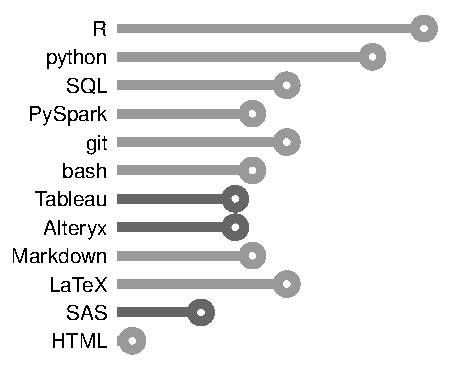
\includegraphics[width=\maxwidth]{figure/skills_plot-1} \hfill{}



\end{knitrout}
    
	\normalsize \toolboxitem{lightgray}{statistics} \\ \footnotesize
	Bayesian methods (RStan) $\cdot$
	hierarchical models $\cdot$
	mixture models $\cdot$
	multivariate statistics $\cdot$
	ANOVA $\cdot$
	MANOVA $\cdot$
	PERMANOVA $\cdot$
	dimensionality reduction $\cdot$
	repeated measures \\
	
  \vspace{-6mm} 
  \normalsize \toolboxitem{lightgray}{supervised learning} \\ \footnotesize
  random forest $\cdot$
  time series $\cdot$
  linear, nonlinear, logistic regression $\cdot$
  LDA $\cdot$
  SEM \\

  \vspace{-6mm} 
  \normalsize \toolboxitem{lightgray}{unsupervised learning} \\ \footnotesize
  PCA $\cdot$
  k-means $\cdot$
  feature engineering
}

%----------------------------------------------------------------------------------------
%	 ACHIEVEMENTS
%----------------------------------------------------------------------------------------
\addachievements{
        \achievementitem{Sustainability Leadership Fellow}{2017-2018}{Colorado State University}{
        {
\includegraphics[width=\logosize, height=\logosize]{csu}} % logo
        } % 25\% acceptance rate
        \achievementitem{Vice President for Research Fellow}{2016-2017}{Colorado State University}{
        {
\includegraphics[width=\logosize, height=\logosize]{csu}} % logo
        } % <10\% acceptance rate
        \achievementitem{18 peer-reviewed publications}{2010-2020}{\textcolor{special}{\href{https://scholar.google.com/citations?user=k6RyLHsAAAAJ&hl=en}{Google Scholar}}}{
        \faBook % logo
        }
}

%----------------------------------------------------------------------------------------
%	 EXPERIENCE
%----------------------------------------------------------------------------------------
\addexperience{

       \experienceitem{Fred Hutch Cancer Center}{Senior Staff Scientist}{07/2022 - present}{Seattle, WA (remote)}{
          \item Led \$579k NIH-funded program (\textcolor{special}{\href{https://reporter.nih.gov/search/RBdFWQthTk2yA8DWBOpd8g/project-details/10854368}{"GEMs"}}) to democratize genomics education through scalable genomic data science training modules, directing collaboration between research institutions and under-resourced colleges
          \item Developed and taught \$200k/yr \textcolor{special}{\href{https://daseh.org}{Data Science for Environmental Health program}}, educating ~40 trainees and public health government professionals annually
       }{hutch} \\
       \vspace{1mm}

       \experienceitem{Johns Hopkins University}{Faculty Associate}{05/2021 - present}{Baltimore, MD}{
          \item Taught grad-level \textcolor{special}{\href{https://jhudatascience.org/intro_to_r/}{Introduction to R for Public Health Researchers}} (7x), including wrangling, stats, and visualization essentials
          \item Taught grad-level \textcolor{special}{\href{https://jhudatascience.org/Baltimore_Community_Course}{Baltimore Community Data Science}} (2x): consulting-like service learning course that partners with community organizations to meet their data-related needs 
       }{jhu} \\
       \vspace{1mm}

       \experienceitem{Johns Hopkins University}{Postdoctoral Fellow}{03/2020 - 05/2020}{Baltimore, MD}{
          \item Led the Urban Evolution Comparative Study, quantifying how 1000+ plants adapted to 6 city landscapes at the genomic level
       }{jhu} \\
       \vspace{1mm}

        \experienceitem{Boston Consulting Group}{Data Scientist}{03/2019 - 03/2020}{Boston, MA}{
           \item Productionalized PySpark pipeline describing client's 20K+ commercial banking customers for better product recommendations \& risk intervention
           \item Designed \& hosted fully customized RShiny dashboard for reducing internal carbon emissions by 30\% in 5 years
        }{gamma} \\
        \vspace{1mm}
      
      %--------------------
      %	 EXPERIENCE Plot
      %--------------------
            
\begin{knitrout}
\definecolor{shadecolor}{rgb}{0.969, 0.969, 0.969}\color{fgcolor}

{\centering 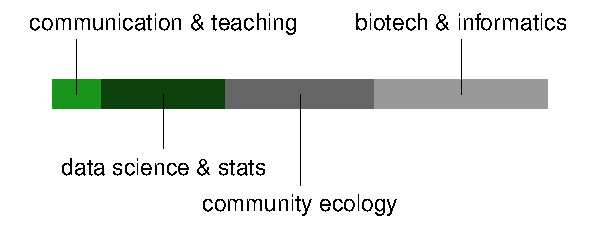
\includegraphics[width=\maxwidth]{figure/experience_plot-1} 

}



\end{knitrout}
      \vspace{-30mm}   

}


%----------------------------------------------------------------------------------------
%	 SECOND PAGE 
%----------------------------------------------------------------------------------------
\clearpage
\printheader

\vspace{9mm}

%----------------------------------------------------------------------------------------
%	 SECOND PAGEEXPERIENCE
%----------------------------------------------------------------------------------------

\addexperienceonly{

        \experienceitem{Insight Data Science}{Data Science Fellow}{09/2018 - 03/2019}{Remote Program}{
            \item Developed and launched \textcolor{special}{\href{https://github.com/avahoffman/Natural_parks}{National Perks Project}} to improve National Park visitor experience, modeling crowds over 500+ months \& accommodating user preferences
            \item Built a fully customized web app using Git, Python, \& Flask, providing visitors with actionable recommendations \& access to further resources
        }{insight} \\
        \vspace{1mm}

        \experienceitem{Colorado State University}{USDA NIFA Fellow}{01/2017 - 12/2018}{Fort Collins, CO}{
        \item Proposed \& established the \textcolor{special}{\href{https://github.com/avahoffman/blue-grama-diversity}{Blue Grama Diversity Project}} to reveal genetic diversity \& guide conservation in a key grass species, while communicating take-home facts to the Front Range non-science community
        \item Pioneered genomic sequencing \& population delineation using 9,000+ genomic features
        \item Modeled hierarchical linkages between genomics, populations, \& plant traits, developing analytical workflows using R \& RStan
        }{nifa} \\
        \vspace{1mm}
}

\cheekyfooter{I built this resume using LaTeX and R. My code can be found \textcolor{special}{\href{https://github.com/avahoffman/CV-and-resumes}{here}}.}

%%%%%%%%%%%%%%%%%%%%%%%%%%%%%%%%%%%%%%%%
\end{document} 
